\documentclass[12pt]{article}
\usepackage[utf8]{inputenc}
\pagenumbering{arabic}
\usepackage{graphicx}
\usepackage{amstext}
\usepackage[usenames, dvipsnames]{color}
\usepackage{array}
\usepackage{float}
\usepackage{enumitem}
\usepackage[top=1.5in]{geometry}
\usepackage{subcaption}
\graphicspath{ {images/} }


\begin{document}

\begin{titlepage}
    \begin{center}
    \begin{figure}
        \centering
        
\includegraphics[scale=0.2]{logoPolimi.png}
        \vspace{1.5cm}
    \end{figure}

    \Huge\textbf{Software Engineering 2 Project - Travlendar+}
    \rule{12cm}{0.5pt}
    \Huge\textbf{Requirement Analysis and Specification Document - V1.2}
    \today
    \end{center}
    
    \vspace{3cm}
    
    \begin{flushleft}
        \LARGE\textbf{Authors: }
        \newline\newline
        \Large\texttt{}{Francisco Cristóvão \\ Samsom Tsegay Beyene}
    \end{flushleft}



\end{titlepage}

\newpage
  \tableofcontents
\newpage

\section{Introduction}

\subsection{Purpose}

The main goal of this project is to create a calendar-based system which provides the user a flexible and fully-featured calendar support that considers the travel time between meetings. With this in mind, the application will:
\begin{itemize}
\item Compute and account for travel time between appointments, and prevent conflicts between them.
\item Support the user in his/her travels, adding automatically the travel time to the calendar between meetings, and suggesting the best travel option based on the available time.
\item Plan the User schedule in the best and most efficient way.
\end{itemize}

\subsection{Scope}
Travlendar+ is a calendar-based application that provides the user a convenient way of organizing his/her daily schedule, maximizing its productiveness and minimizing the worthless time of his/her day. This application was not only thought for the regular businessman/businesswoman, who travel in between meetings the whole day and have no time to spare, but also for the parents with a more regular daily schedule, who just want to get the best out of their time while being able to pick their kids from school and take them to other activities, always being on time.
Of course the system will fully support the features of a regular calendar application (booking of appointments in a specific time and location), but in a "smart" way, being able to detect and warn the user if a new appointment is not feasible because it has a conflict (the start of it doesn't allow the needed travel time after the end of the last appointment) and arranging all of the appointments in the best possible way. The application is meant to be used in the City of Milan, and so it will take advantage of the wide range of travel means and services already existing in the city, from public transports to shared bikes and cars. With the information gathered from those services, it will be able to suggest the best travel mean for the user to move between appointments, based on the available travel time, total cost, current weather and even user preferences.


\subsection{Definitions, Acronyms, Abbreviations}
\subsubsection{Definitions}
\textit{Visitor}: A person who uses Travlendar+ for the first time, and is not yet registered.\\
\textit{User}: A person who uses Travlendar+.\\
\textit{Home Screen}: User interface screen that shows the current appointments.\\
\textit{Flexible Appointment}: An appointment which the start and end date may change between a given time range (are flexible), as long as its minimum duration is ensured.\\
\textit{System}: defines the overall set of software components that implement the required functionality.\\
\textit{Local Time}: time of the system.
\subsubsection{Acronyms}
\textit{API}: Application Programming Interface\\
\textit{RASD}: Requirements Analysis and Specification Document\\
\textit{ATM: Azienda Trasporti Milanesi}\\
\textit{SQL}: Structured Query Language\\
\textit{BPMN}: Business Process Model and Notation
\subsubsection{Abbreviations}
\textit{Gn}: Goal defined with index n.\\
\textit{Dn}: Domain Assumption defined with index n.\\
\textit{Rn}: Functional Requirement defined with index n.


\subsection{Revision History}
\textbf{Version 1.1:} 
\begin{itemize}
    \item Fixed a number of typos all over the document.
    \item Added the "Change Password" use case to the user use case diagram.
    \item Changed the layout of some buttons on the User Interfaces.
    \item Added Domain Assumption 13 to better cover all of the possible situations when an appointment can be created: 
        \begin{itemize}
            \item When there are no previous appointments in that day, the system assumes that the location from where the user is going to the appointment is his house
        \end{itemize}
    \item Added Domain Assumption 14 to better cover all of the possible situations when an appointment can be created: 
        \begin{itemize}
            \item When there are no further appointments in that day, the system assumes that the location where the user is going after the appointment is his house.
        \end{itemize}
    \item Added Domain Assumption 15 since it is a reasonable assumption that fits the requirements and highly simplifies the appointment management: 
        \begin{itemize}
            \item The possible interval for a flexible appointment cannot be overlapped by the possible interval for another flexible appointment, even if there's enough space for the minimum duration of both.
        \end{itemize}
    \item Modified Goal 1 to better express what the system is intended to do: 
        \begin{itemize}
            \item Allow only registered users to access the most relevant functionality of the system.
        \end{itemize}
    \item Modified Goal 1 to include the following requirement (R4):
        \begin{itemize}
            \item The system shall not allow a visitor to access more than the registration functionality.
        \end{itemize}
    \item Modified the Alloy model in order to meet the changes in the domain assumptions, more specifically the Domain Assumption 15:
        \begin{itemize}
            \item Changed the way the flexible appointments where modeled: they now contemplate the existence of a "real" start and end time, where the appointment is scheduled, and a start and end time for the interval where the appointment can be scheduled.
            \item Added some facts to manage the restrictions of this new representation.
            \item Changed the generated worlds in order to meet the changes in the Alloy model.
        \end{itemize}
\end{itemize}
\textbf{Version 1.0:} Initial Release
\subsection{Reference Documents}
    \begin{itemize}
        \item Assignment document: Mandatory Project Assignments.pdf
        \item IEEE Recommended Practice for Software Requirements Specifica- tions (Std 830-1998)
    \end{itemize}


\subsection{Document Structure}
Other than this introductory chapter, this RASD is organized in six more chapters. Chapter two is meant to provide an overview of the system's functionality, the type of users it is meant for and the different kinds of interactions it contemplates, not only with the users themselves but also with other systems. Some of the systems requirements are also slightly discussed in this chapter, even though they’ll be analyzed in the following chapter. In the third chapter (as mentioned) the system requirements, attributes and constraints are analyzed and discussed in the appropriate detail and depth, specifying exactly how they should be.
The fourth chapter deals with the formal analysis of the system using an Alloy model. It includes the Alloy model of the system with a brief discussion on its purpose and on the relevance of using Alloy as a tool to validate our solution, given the problem we had to solve.
In the fifth chapter the effort spent by each of the group members is described by specifying the number of hours each member of the group worked on the development of this document, and on the final chapter the tools we used to develop this RASD are specified.

\section{Overall Description}

\subsection{Product Perspective}
The system will need to communicate with both public transport systems, bike or car sharing system of the city and Google maps API to find the exact status of available (active) types of transportation with their corresponding locations. These information helps the System to exactly locate the position of the user and the appointments place so that it can assign the best travel means to get to the referred appointment. In addition, the System also retrieves the weather conditions and takes them into consideration when choosing the travel mean.
Since this system relies on data storage to work, it will need some alternative to store this data. So, the system will communicate with the database (probably distributed) to add or modify the appointments, as well as the user details and preferences. All the database communication will go over the Internet.
    \begin{figure}[H]
        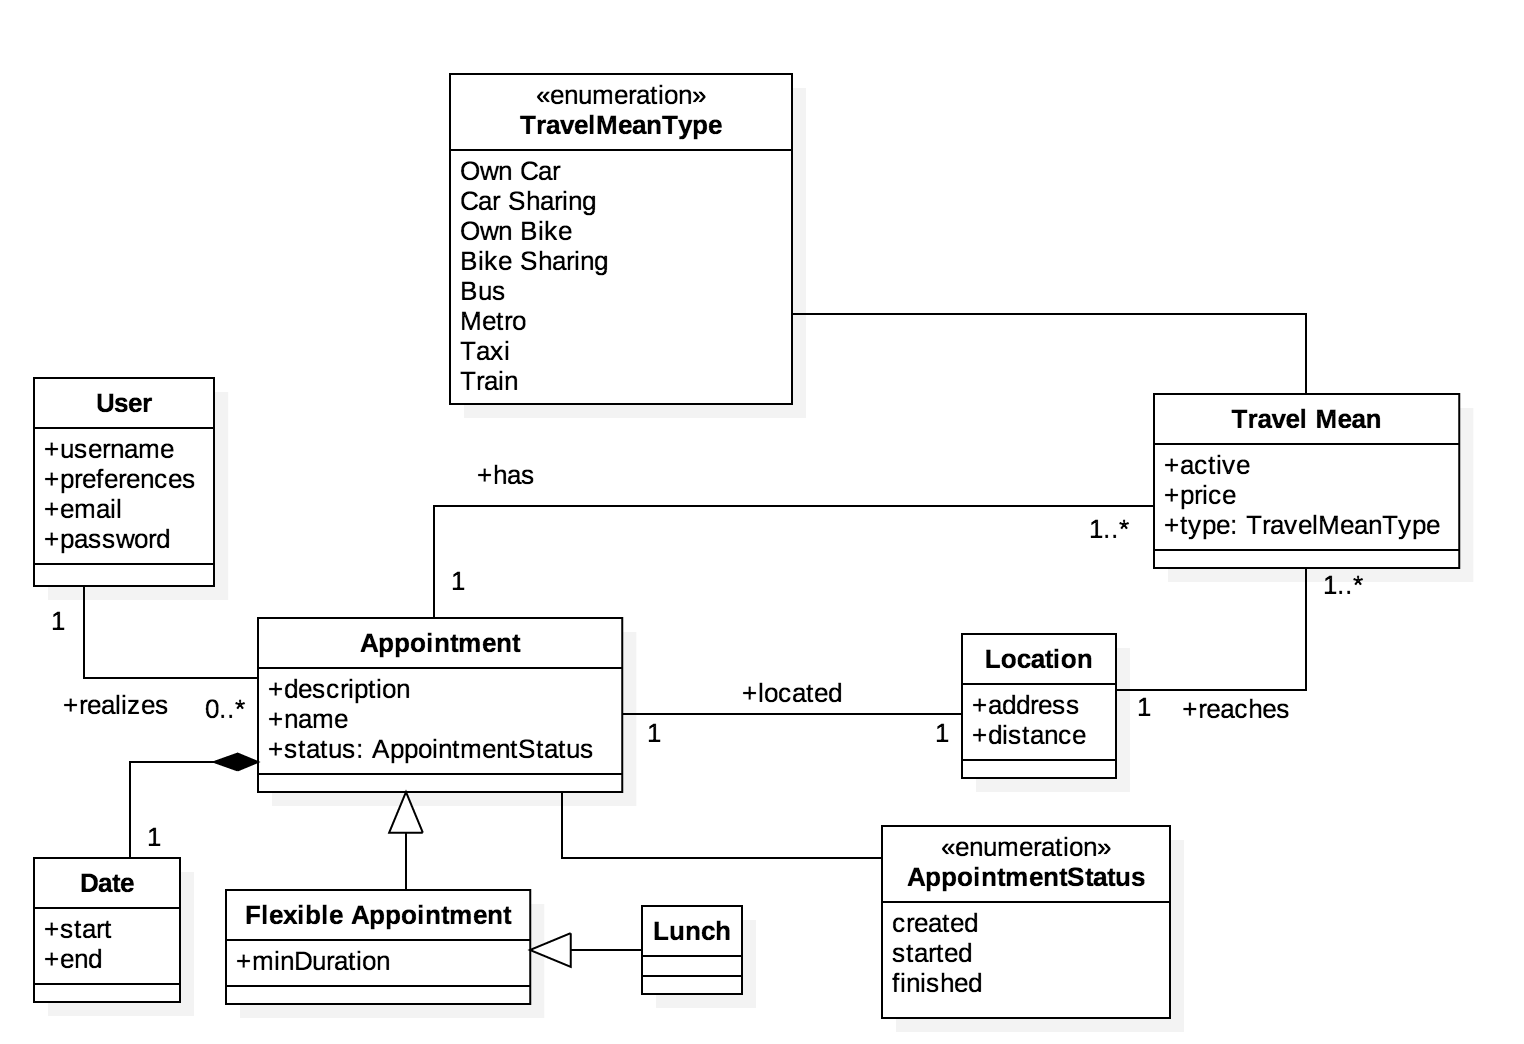
\includegraphics[scale=0.3]{domainModel.png}
        \caption{Class Diagram of the domain}
        \centering
    \label{fig:domainModel}
    \end{figure}
    \begin{figure}[H]
    \centering
        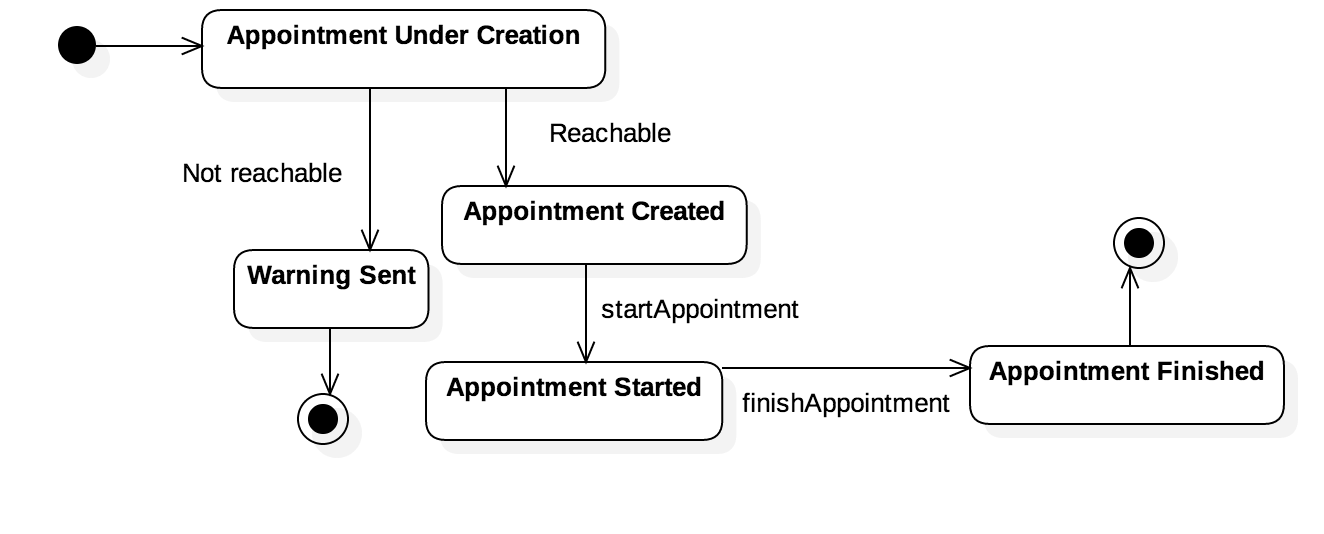
\includegraphics[scale=0.33]{statechartAppointment.png}
        \caption{Statechart of an Appointment}
    \label{fig:domainModel}
    \end{figure}
    
\subsection{Product Functions}
The main functions supported by the system will be:
\begin{itemize}
    \item Allow the user to book an appointment with a given time, location and duration.
    \item Plan the user's schedule in the best possible way, choosing for him where to place flexible appointments and suggesting which travel means to use in between appointments, based on his preferences, the time available and the weather.
\end{itemize}

\subsection{User Characteristics}
The system aims at satisfying the needs of many different types of users. The first type is the "businessman" user, the user that is always in a tight schedule and needs a tool like our system to simplify and improve the way he organizes his schedule and the way turns up to the appointments. The second type is the opposite of the "businessman" user. It's a user that has a less busy life and only needs the system to remind him of the appointments without having to worry about how to get there or when to leave to arrive on time. There's also a third type of user which is placed in between the two described previously: also has a tight office schedule but still has time for personal activities, and needs the system to help him reach this balance in the most efficient way.
All of these types of users are of working age (20 to 70 years old, being this a small deviation of the official definition, which is from 15 to 64 years old)\footnote{Definition from OECD: https://data.oecd.org/pop/working-age-population.htm} and are expected to know how to use a smartphone with reasonable proficiency. It's easy to see that the needs of the users will map directly to the goals of the system, most precisely to G5, which is the more general and "different" from the similar applications already on the market, and the one the users are looking more forward to.

\subsection{Assumptions, dependencies and constraints}
[D1] The username and email must be unique.\\{}
[D2] The system will have access to the phone GPS functionality.\\{}
[D3] The phone will always have a connection to the internet (WiFi or mobile data).\\{}
[D4] The best route and travel mean to get to an appointment will always be computed correctly.\\{}
[D5] The users authorize the system to provide user data (when needed) to the third-party applications it interacts with.\\{}
[D6] The external services used by the system are assumed to be always available and reachable.\\{}
[D7] Changes on the user preferences only apply to the appointments created after the change. The ones already created stay the same.\\{}
[D8] Two different users are not allowed to interact with each other. For example, even though two users are meeting each other, the system won't recognize the relation between meetings and will considered them as two different meetings.\\{}
[D9] The best travel means to get to an appointment won't change if the appointments don't change.\\{}
[D10] Users don't need to confirm if they started or finished the appointment.\\{}
[D11] An Appointment maps to only one User.\\{}
[D12] The location of the users private car and bike is always known by the system.\\{}
[D13] When there are no previous appointments in that day, the system assumes that the location from where the user is going to the appointment is his house.\\{}
[D14] When there are no further appointments in that day, the system assumes that the location where the user is going after the appointment is his house.\\{}
[D15] The possible interval for a flexible appointment cannot be overlapped by the possible interval for another flexible appointment, even if there's enough space for the minimum duration of both.\\{}\\{}
\textbf{N.B.:} D15 was considered because if we considered that flexible and fixed appointments could overlap other flexible appointment's possible scheduling interval, the algorithm to manage the appointments would be really complex to implement and would provide extra functionally that is in some sort of way unnecessary given the domain of our system, more specifically the goal of having flexible appointments (the difference in complexity wouldn't justify the difference in functionality)


\section{Specific Requirements}

\subsection{External Interface Requirements}

\subsubsection{User Interfaces}
These Mockups represent a basic idea of how the systems user interface will look like on the first release (mobile application):

\begin{figure}[H]
\centering
    \begin{subfigure}{.4\textwidth}
        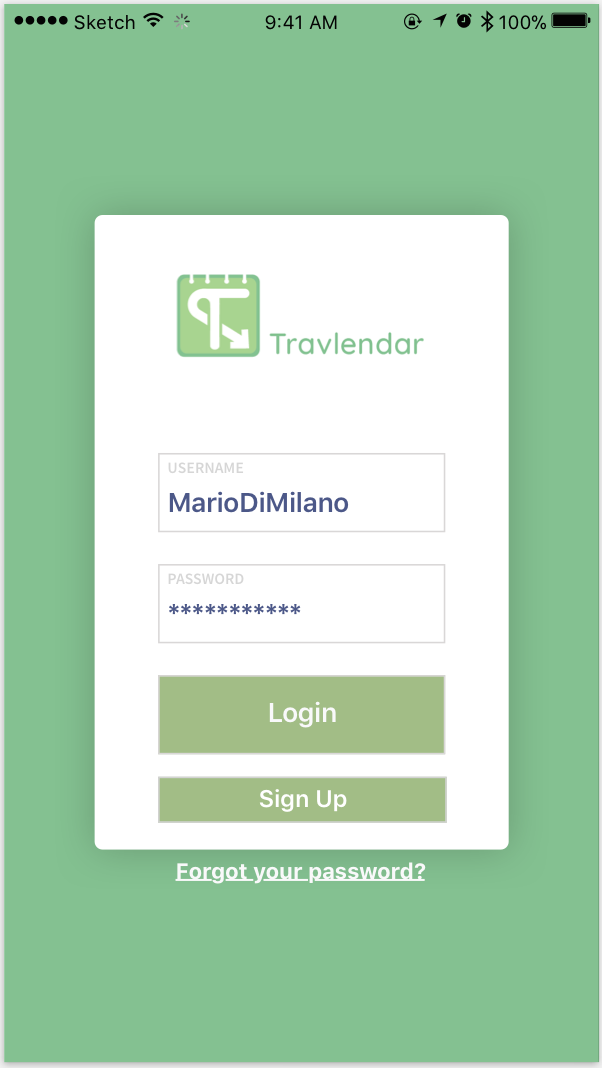
\includegraphics[scale=0.44]{interfaceLogin.png}
        \label{fig:loginScreen}
    \end{subfigure}%
    \begin{subfigure}{.4\textwidth}
        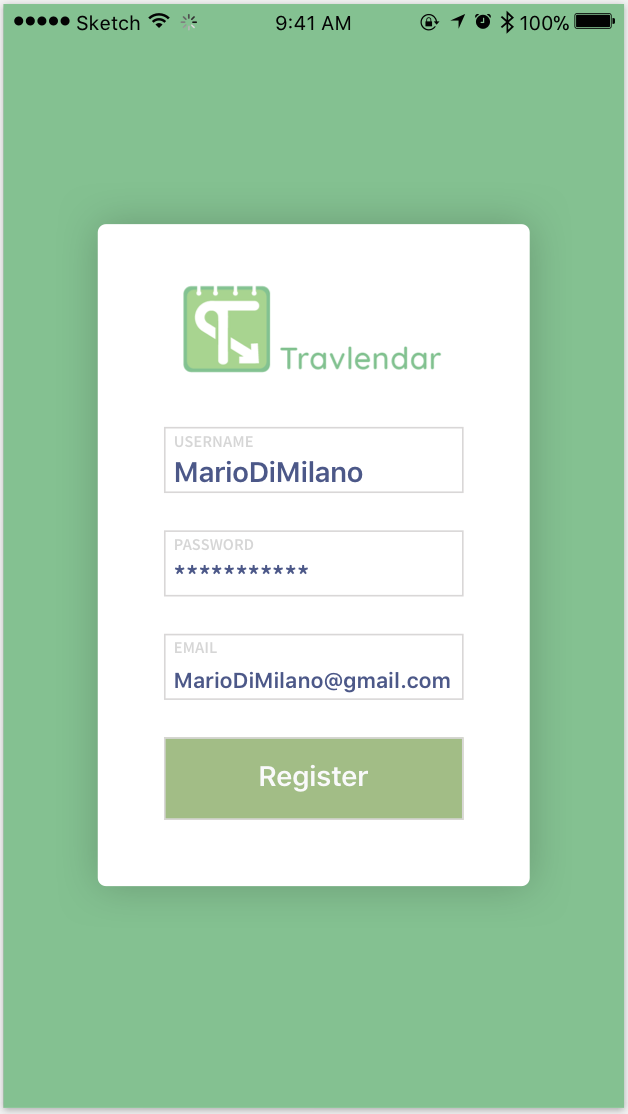
\includegraphics[scale=0.44]{interfaceRegister.png}
        \label{fig:registerScreen}
    \end{subfigure}
    \caption{Login Screen (left) and Register Screen (right)}
\end{figure}

\begin{figure}[H]
\centering
    \begin{subfigure}{.4\textwidth}
        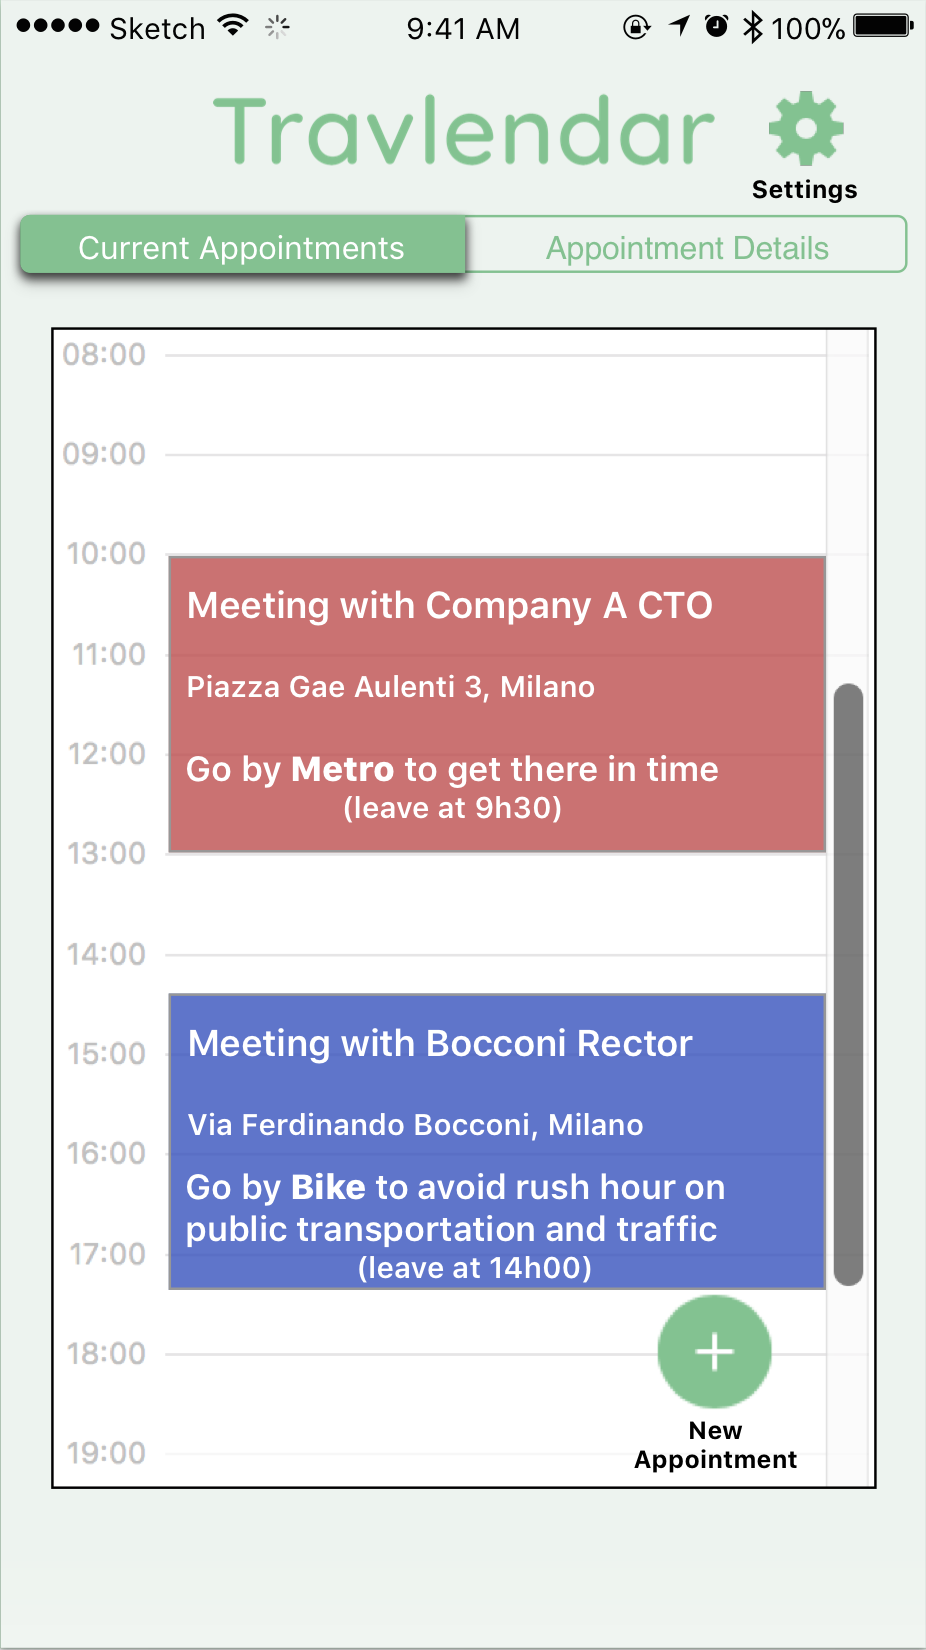
\includegraphics[scale=0.445]{interfaceHome.png}
        \label{fig:homeScreen}
    \end{subfigure}%
    \begin{subfigure}{.4\textwidth}
        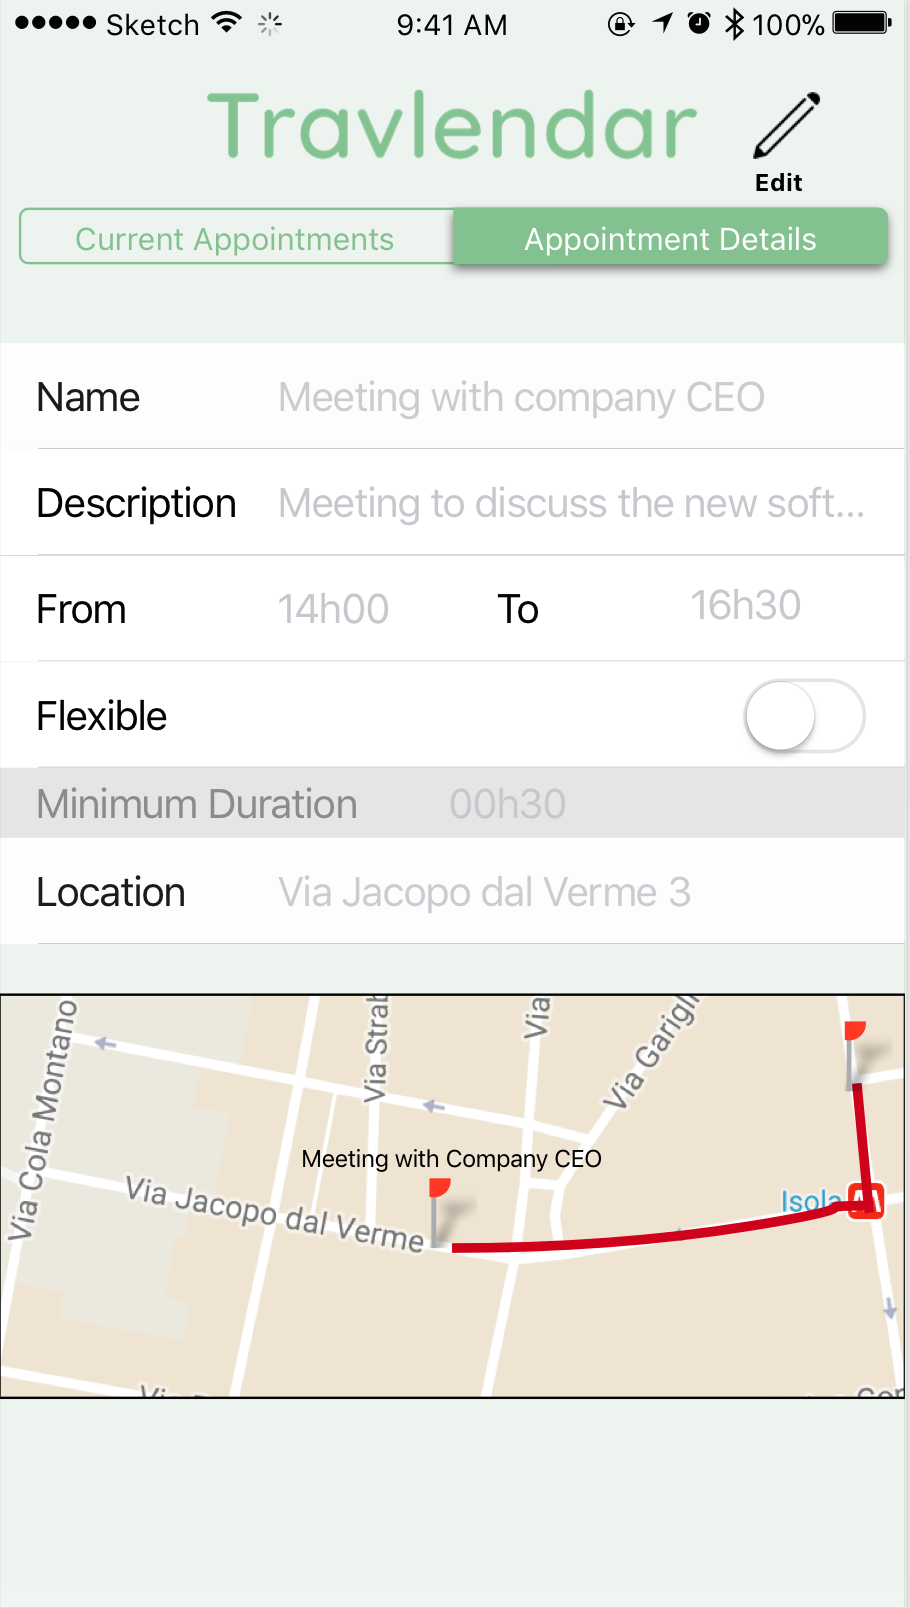
\includegraphics[scale=0.44]{interfaceAppointment.png}
        \label{fig:newAppointmentScreen}
    \end{subfigure}
    \caption{Home Screen (left) and Appointment Details Screen (right)}
\end{figure}

\begin{figure}[H]
\centering
    \begin{subfigure}{.4\textwidth}
        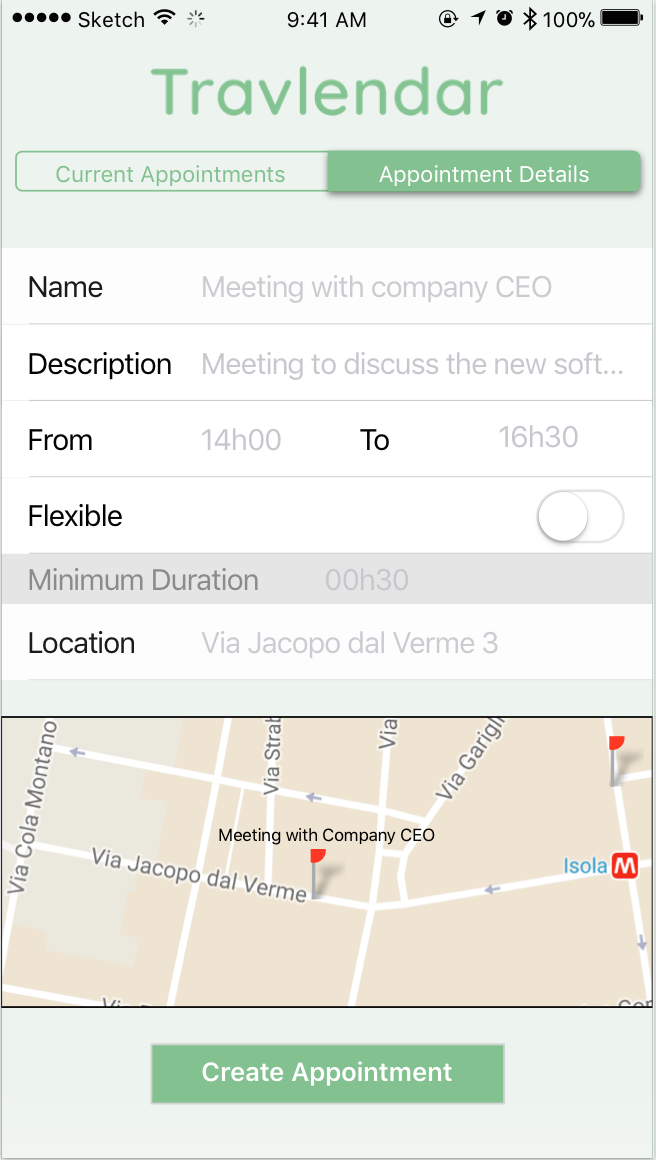
\includegraphics[scale=0.44]{interfaceNewAppointment.png}
        \label{fig:appointmentScreen}
    \end{subfigure}%
    \begin{subfigure}{.4\textwidth}
        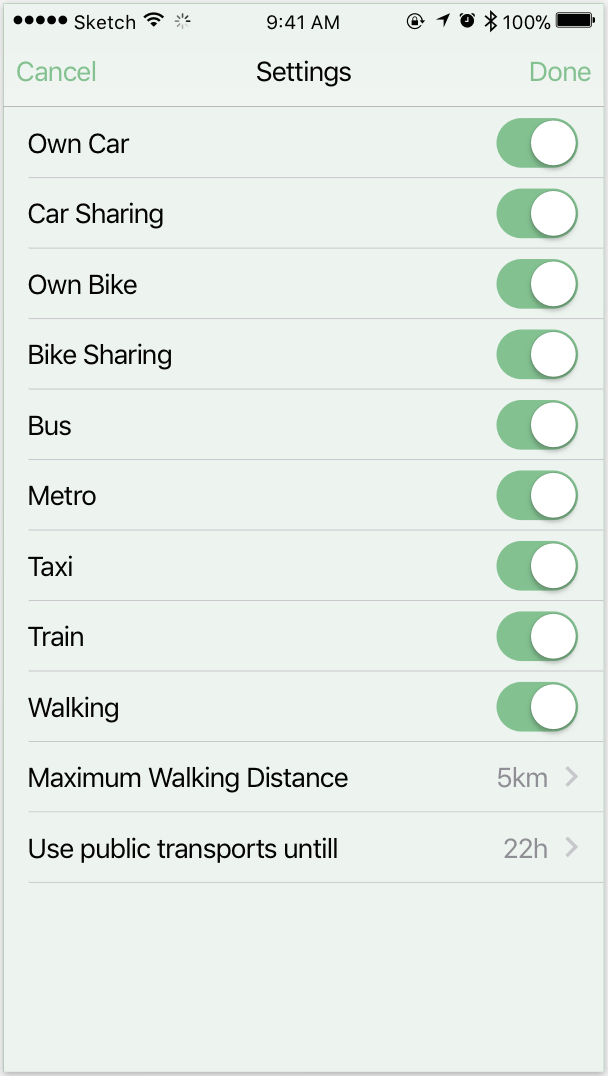
\includegraphics[scale=0.455]{interfaceSettings.png}
        \label{fig:settingsScreen}
    \end{subfigure}
    \caption{New Appointment Screen (left) and Settings Screen (right)}
\end{figure}


\subsubsection{Hardware Interfaces}
In the first release, no Hardware Interfaces will be necessary since the system doesn't need to interact physically with other systems.

\subsubsection{Software Interfaces}
Given the wide range of features the system offers, it will need to have several software interfaces. There has to be a way of storing all the user-related data (mainly login, preferences and appointments data). In that sense, the system will use a \textbf{MySQL API} to connect with a MySQL database server, where all the app data will be stored.\\
The system will also need different kinds of information about the users location and its surrounding, in order to compute the travel time between appointments. To support this functionality, the system will use \textbf{Google Maps Geolocation API} and \textbf{Google Maps API}. The first one will provide information about the user exact location and the second one will provide the real-time information about maps and traffic, and allow it to calculate the best route between two different appointments.\\
To have access to the current weather, the system will use \textbf{AccuWeather API}, which will provide information about the current weather on both where the user is and where the appointment is located.
At last, the system will also need to get all sorts of information from many different travel means. In order to get this information, it will have a software interface with \textbf{ATM Milano} (public transport schedule and routes), \textbf{Drive Now API} (for the car sharing system) and \textbf{Mobike API} (for the bike sharing system).



\subsubsection{Communication Interfaces}
Communication interfaces ensure the communication between the system and the other software interfaces (third party service providers).
The communication between the system and those service providers is crucial because the system depends on those services to perform its functions. Given this, the systems communication interface must be either WiFi or Mobile Data (2G, 3G or 4G), and the service providers communication interface can be of any type, as long as it ensures that they are connected to the internet. The protocol used shall be HTTPS, in order to keep the communications secure.

\subsection{Functional Requirements}

{[G1]} Allow only registered users to access the most relevant functionality of the system.
\begin{itemize}
    \item{[R1]} The system shall allow the visitor to begin the registration process when he accesses the system. 
    \item{[R2]} The system shall ask the visitor for the required information and credentials during the registration process.
    \item{[R3]} The system shall register the visitor as a user when the registration process ends, if all the data inserted by the user is valid.
    \item{[R4]} The system shall not allow a visitor to access more than the registration functionality.
\end{itemize}
{[G2]} Allow a logged user to create an appointment.
\begin{itemize}
    \item{[R5]} The system shall allow the user to fill in all the needed information about the appointment.
    \item{[R6]} The system shall not allow two appointments to overlap.
    \item{[R7]} The system shall create a warning if the appointments location is unreachable.
    \item{[R8]} The system shall not allow the user to create an appointment if the location is unreachable.
    \item{[R9]} The system shall allow the user to select if the appointment is flexible or not.
    \item{[R10]} The system shall create the appointment if all the data inserted by the user is valid.
\end{itemize}

{[G3]} Allow a logged user to edit an appointment.
\begin{itemize}
    \item{[R11]} The system shall allow the user to edit all the provided information about the appointment.
    \item{[R6]} The system shall not allow two appointments to overlap.
    \item{[R7]} The system shall create a warning if the appointments new location is unreachable.
    \item{[R12]} The system shall not allow the user to submit the changes if the new location is unreachable.
    \item{[R13]} The system shall submit the changes to the appointment if all the data inserted by the user is valid.
\end{itemize}
{[G4]} Allow a logged user to delete an appointment.
\begin{itemize}
    \item{[R14]} The system shall allow the user to delete all the data related to the appointment that the user wants to delete.
\end{itemize}
{[G5]} Allow a logged user to have his schedule planned in the best possible way.
\begin{itemize}
    \item{[R15]} The system shall compute the best possible arrangement of the users appointments that fulfills his/her preferences.
    \item{[R6]} The system shall not allow two appointments to overlap.
    \item{[R16]} The system shall compute the best travel mean to get to each appointment.
    \item{[R17]} The system shall re-plan the users schedule every time an appointment is inserted, deleted or its location and/or date is changed.
    \item{[R18]} The system shall re-compute the best travel mean to get to the other appointments in case one of the appointment gets deleted or its location is edited.
    \item{[R19]} The system shall display the best travel mean to get to each appointment, along with the best arrangement of appointments.
    
\end{itemize}
{[G6]} Allow a logged user to define preferences related to travel means.
\begin{itemize}
    \item{[R20]} The system shall allow the user to enable all the travel means he wants the system to consider when computing the best way to move in between appointments.
    \item{[R21]} The system shall allow the user to disable all the travel means he doesn't want the system to consider when computing the best way to move in between appointments.
    \item{[R22]} The system shall allow the user to select the maximum distance he is willing to walk from one appointment to another.
    \item{[R23]} The system shall allow the user to select an hour of the day from when public transportation shall not be used.
    \item{[R24]} The system shall allow the user to select a combination of public transportation in order to minimize his carbon footprint (includes only walking, bike or electric travel means).
\end{itemize}

\newpage
\subsubsection{Use Case Diagrams}


\begin{figure}[H]
        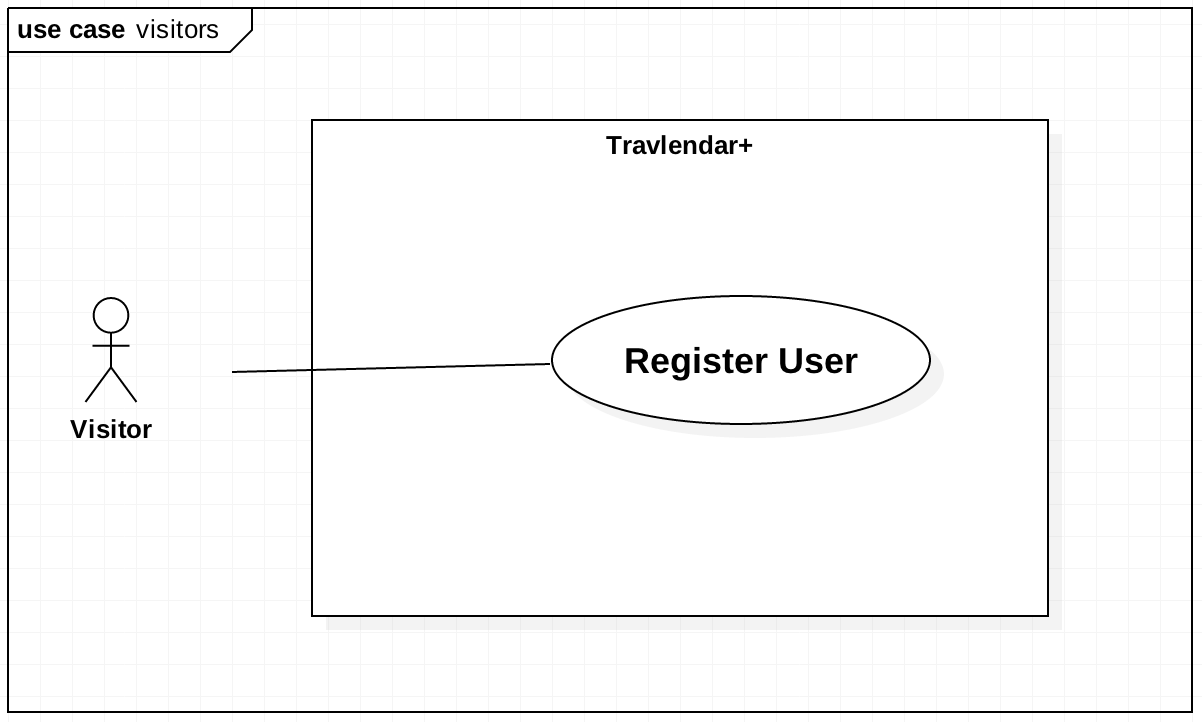
\includegraphics[scale=0.4]{visitorUseCase.png}
        \centering
        \caption{Visitor Use Case}
    \label{fig:visitorUseCase}
\end{figure}


\begin{figure}[H]
        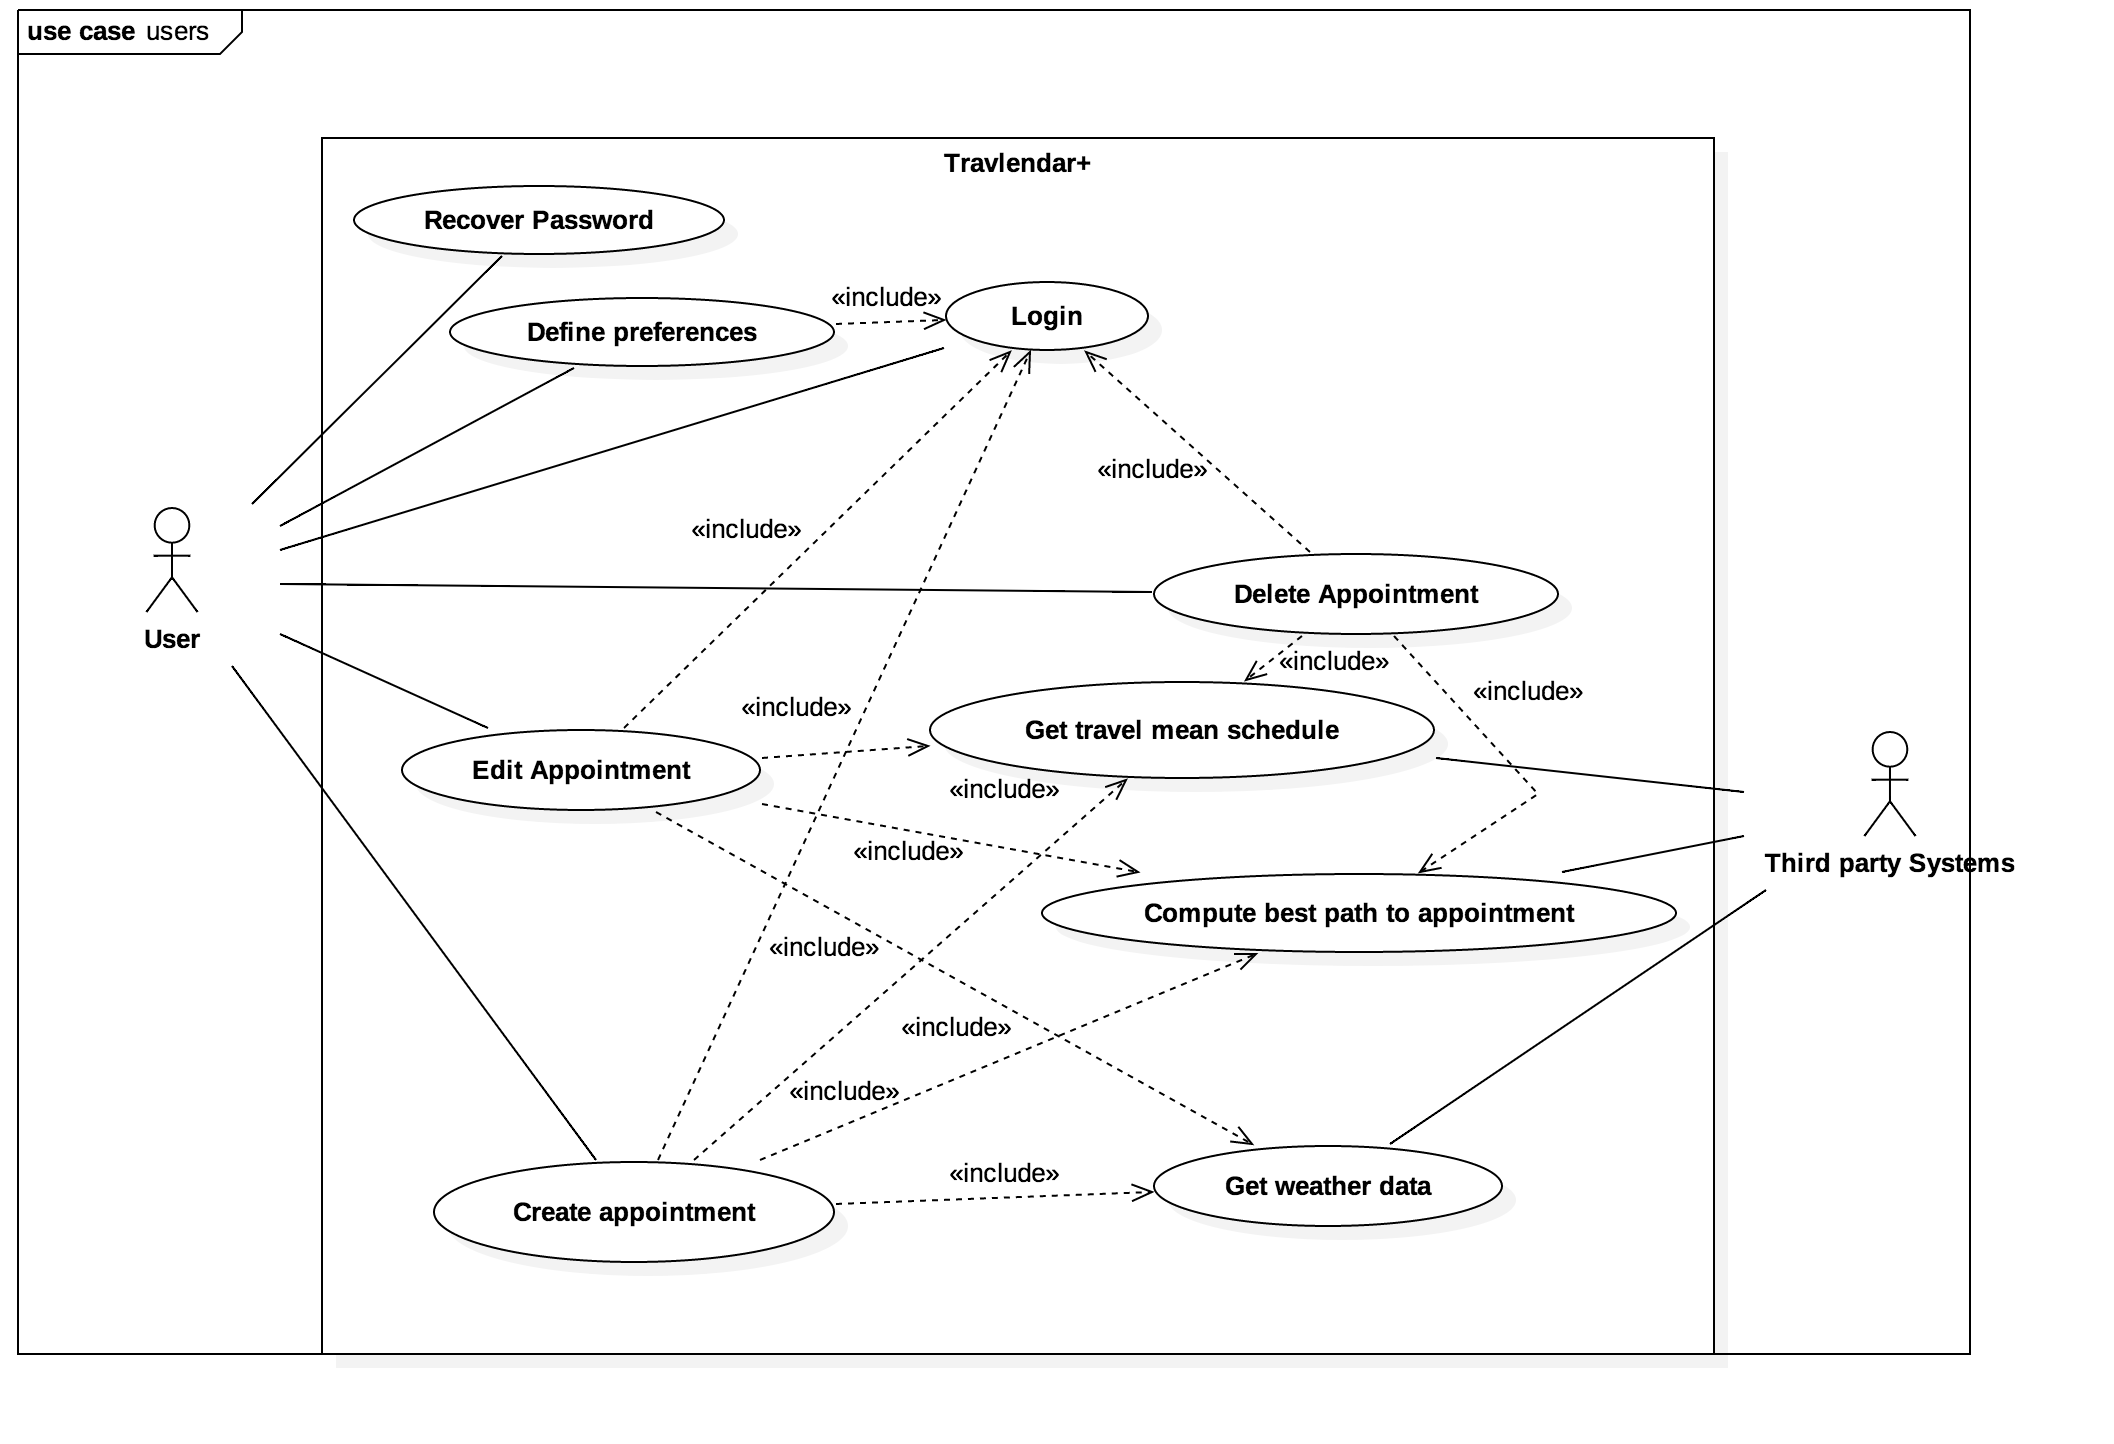
\includegraphics[scale=0.23]{userUseCase.png}
        \centering
        \caption{User Use Case}
    \label{fig:userUseCase}
\end{figure}
    
\newpage

\subsubsection{Use Case Description}
\paragraph{Visitor Registration}

\begin{center}
    \begin{tabular} { |p{0.25\textwidth}|p{0.7\textwidth}| }
        \hline
        \textbf{Actors} & Visitor \\ 
        \hline
        \textbf{Goals} & {[G1]} \\ 
        \hline  
        \textbf{Preconditions} & There are no preconditions. \\ 
        \hline
        \textbf{Events Flow} & \begin{enumerate}[topsep=0pt]
                            \setlength{\itemsep}{0.5pt}
                            \item The visitor opens Travlendar+ application.
                            \item The visitor clicks on the "Sign up" button to start the registration process.
                            \item The system provides the Visitor a form with the required data fields which need to be filled in order for him to be registered as a user.
                            \item The visitor fills the fields with his data. 
                            \item The visitor clicks on the "Register Button", submitting the data to the system.
                            \item The system verifies if all the data are valid.
                            \item The system saves the data.
                            \item The system notifies the Visitor that his registration as a user has been completed with success, and redirects him to the Home Screen
                            \end{enumerate} \\
        \hline
        \textbf{Postconditions} & The visitor ends the registration process successfully and from now on is a user of the system, being able to access all of its functionality. \\
        \hline
        \textbf{Exceptions} & \begin{enumerate}[topsep=0pt]
                            \setlength{\itemsep}{0.5pt}
                            \item The visitor is already a user. 
                            \item The visitor doesn't fill all the mandatory fields or fills them with invalid data.
                            \item The visitor chooses a username or email which is already associated with another user.
                            \end{enumerate} 
                            All exceptions are handled notifying the visitor about the issue and going back to the applications initial screen.\\ 
        \hline
    \end{tabular}
\end{center}

\newpage

\paragraph{User Login}
\begin{center}
    \begin{tabular} { |p{0.25\textwidth}|p{0.7\textwidth}| }
        \hline
        \textbf{Actors} & User \\ 
        \hline
        \textbf{Goals} & All goals except {[G1]} \\ 
        \hline  
        \textbf{Preconditions} & There are no preconditions. \\ 
        \hline
        \textbf{Events Flow} & \begin{enumerate}[topsep=0pt] 
                            \setlength{\itemsep}{0.5pt}
                            \item The user opens Travlendar+ application.
                            \item The user inserts his username and password on the respective fields.
                            \item The user clicks on the "Log In" button.
                            \item The system validates the user credentials.
                            \item The system redirects the user to the Home Screen.
                            \end{enumerate} \\
        \hline
        \textbf{Postconditions} & The user is successfully logged in to the system and redirected to the Home Screen. \\
        \hline
        \textbf{Exceptions} & \begin{enumerate}[topsep=0pt] 
                            \setlength{\itemsep}{0.5pt}
                            \item The user inserts an invalid username or email.
                            \end{enumerate} 
                            All exceptions are handled notifying the User about the issue and going back to event 2 of the Event Flow described above.\\ 
        \hline
    \end{tabular}
\end{center}

\newpage

\paragraph{User creates an appointment}

\begin{center}
    \begin{tabular} { |p{0.25\textwidth}|p{0.7\textwidth}| }
        \hline
        \textbf{Actors} & User \\ 
        \hline
        \textbf{Goals} & {[G2 and G5]} \\ 
        \hline  
        \textbf{Preconditions} & The User must be already logged in. \\ 
        \hline
        \textbf{Events Flow} & \begin{enumerate}[topsep=0pt] 
                            \setlength{\itemsep}{0.5pt}
                            \item The user clicks on the "New Appointment" button
                            \item The system provides the user a form with the required data fields which need to be filled in order for the appointment to be created.
                            \item The user fills the form.
                            \item The user clicks on the "Create Appointment" button.
                            \item The system validates the data.
                            \item The system computes the best new possible arrangement of appointments.
                            \item The system computes the best travel means to get to this new appointment.
                            \item The system saves the data.
                            \item The system redirects the user to the Home Screen.
                            \end{enumerate} \\
        \hline
        \textbf{Postconditions} & The user successfully creates an appointment and continues having the best possible appointment arrangement. \\
        \hline
        \textbf{Exceptions} & \begin{enumerate}[topsep=0pt] 
                            \setlength{\itemsep}{0.5pt}
                            \item The user inserts an invalid Location.
                            \item The user creates an appointment which is unreachable.
                            \end{enumerate} 
                            The exceptions are handled notifying the user about the issue and going back to event 2 of the Event Flow described above.\\ 
        \hline
    \end{tabular}
\end{center}

\newpage

\paragraph{User edits an appointment}

\begin{center}
    \begin{tabular} { |p{0.25\textwidth}|p{0.7\textwidth}| }
        \hline
        \textbf{Actors} & User \\ 
        \hline
        \textbf{Goals} & {[G3 and G5]} \\ 
        \hline  
        \textbf{Preconditions} & The User must have created at least one appointment. \\ 
        \hline
        \textbf{Events Flow} & \begin{enumerate}[topsep=0pt] 
                            \setlength{\itemsep}{0.5pt}
                            \item The user clicks on the appointment he wants to edit.
                            \item The system shows the same form as the one showed when creating an appointment, but with the fields filled with the appointments current data.
                            \item The user clicks on the "Edit" button.
                            \item The user changes the location of the appointment.
                            \item The user clicks on the "Done" button.
                            \item The system validates the data.
                            \item The system computes the best new possible arrangement of appointments.
                            \item The system computes the best travel means to get to the other created appointments, to see if any of those changed with this change.
                            \item The system saves the data.
                            \item The system shows the new arrangement of appointments.
                            \end{enumerate} \\
        \hline
        \textbf{Postconditions} & The user successfully edits an appointment and continues having the best possible appointment arrangement. \\
        \hline
        \textbf{Exceptions} & \begin{enumerate}[topsep=0pt] 
                            \setlength{\itemsep}{0.5pt}
                            \item The user inserts an invalid Location.
                            \item The editing of the location of this appointment makes this or some of the other appointments unreachable.
                            \end{enumerate} 
                            The exceptions are handled notifying the user about the issue (and about which appointments are in conflict if that's the case) and going back to event 2 of the Event Flow described above.\\ 
        \hline
    \end{tabular}
\end{center}

\newpage

\paragraph{User deactivates Bike Sharing as a travel mean}
\begin{center}
    \begin{tabular} { |p{0.25\textwidth}|p{0.7\textwidth}| }
        \hline
        \textbf{Actors} & User \\ 
        \hline
        \textbf{Goals} & {[G6]} \\ 
        \hline  
        \textbf{Preconditions} & The User must be already logged in. \\ 
        \hline
        \textbf{Events Flow} & \begin{enumerate}[topsep=0pt] 
                            \setlength{\itemsep}{0.5pt}
                            \item The user clicks on the "Settings" button
                            \item The system shows a slide button form, one for each mean of transportation.
                            \item The user sets the Bike Sharing slide button to deactivated.
                            \item The User clicks on the "Done" button.
                            \item The System saves the data.
                            \end{enumerate} \\
        \hline
        \textbf{Postconditions} & The user successfully deactivated Bike Sharing as a travel mean and is redirected to the Home Screen. \\
        \hline
        \textbf{Exceptions} & There are no exceptions.\\ 
        \hline
     \end{tabular}
\end{center}

\subsubsection{BPMN Diagrams}

\begin{figure}[H]
        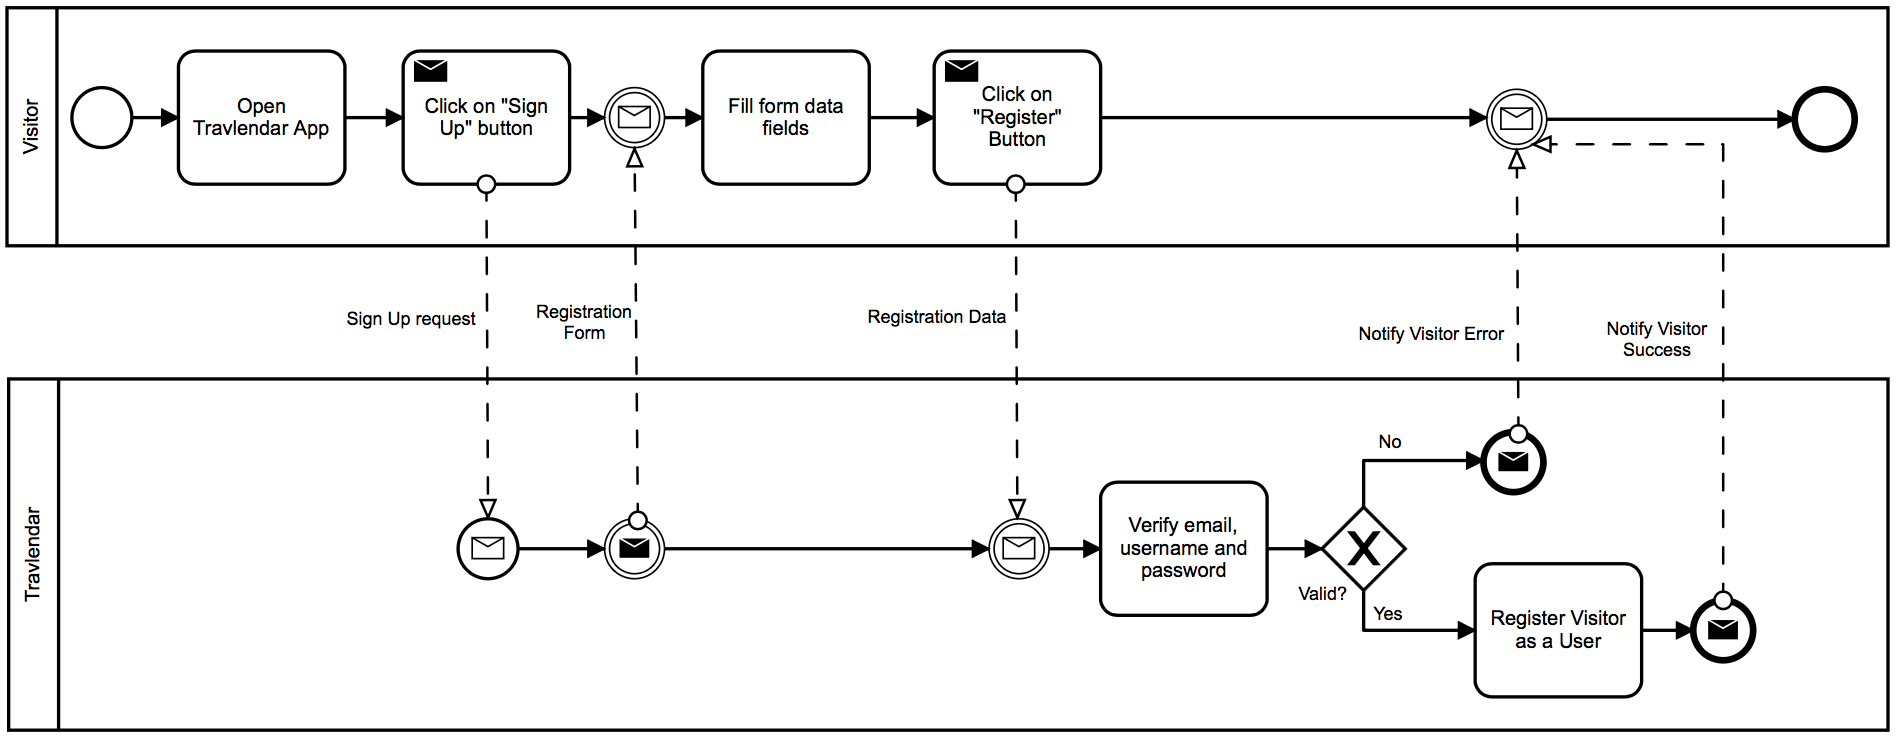
\includegraphics[scale=0.55, angle=-90, origin=c]{BPMNvisitorRegistration.png}
        \centering
        \caption{Visitor Registration}
    \label{fig:visitorRegistrationBPMN}
\end{figure}

\begin{figure}[H]
        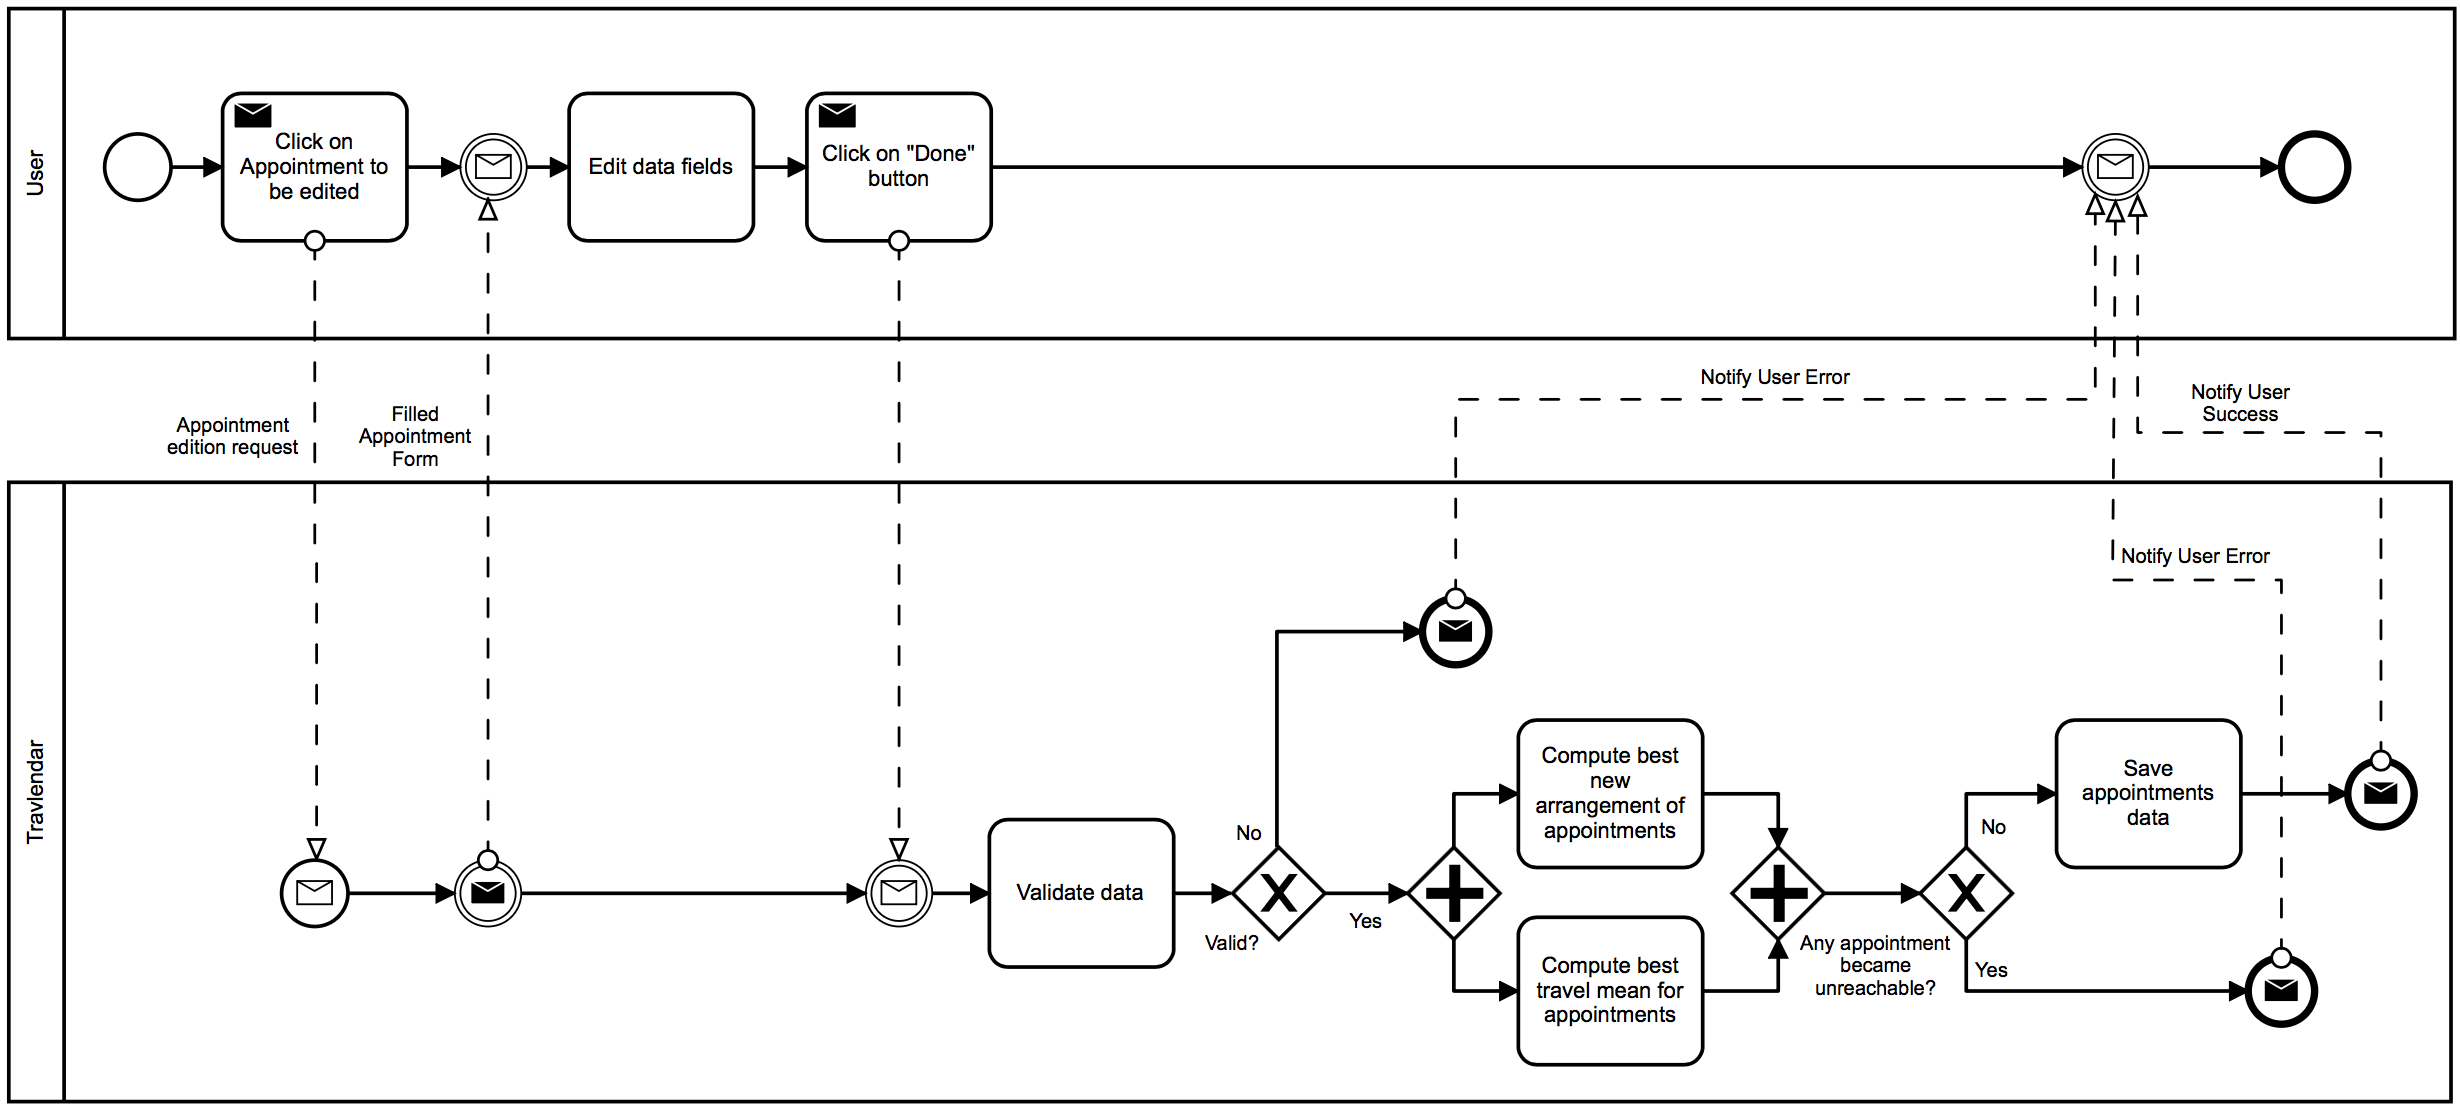
\includegraphics[scale=0.46, angle=-90, origin=c]{BPMNeditAppointment.png}
        \centering
        \caption{User Edits Appointment}
    \label{fig:visitorRegistrationBPMN}
\end{figure}


\subsection{Performance Requirements}
The system has to be able to respond to a possibly large number of requests (depending on the number of users the system will have). Taking into account other (less powerful but widely used) calendar and transport applications, an infrastructure that supports a maximum workload on the order of hundreds of thousands of requests shall be enough to satisfy all the possible simultaneous requests after the release. The infrastructure must have a good scalability in order to increase the maximum workload in case the user base increases too. The response times of the system shall be\footnote{According to Jakob Nielsen book on Usability}:
\begin{itemize}
    \item 0.1 second for the tasks that require almost no computing power (changing menus in the system's case), in order for the user to feel that the system is reacting instantaneously
    \item 1 second for the tasks that require a normal amount of computing power, in order for the user's flow of thought to stay uninterrupted (deleting an appointment in the system's case)
    \item 10 seconds for the tasks that require significant computing power, in order to keep the user's attention (computing the best travel route and consequent travel mean to get to an appointment in the system's case). The users must also receive some sort of feedback during the wait, so they can know what to expect.
\end{itemize}
N.B. A user is assumed to have a stable internet connection in order to achieve these response times.


\subsection{Design Constraints}
\subsubsection{Standard Compliance}
The system must require the user's permission to provide their location, preferences, and schedule to the external services it uses (transport services and weather services), in order to manage sensitive data always respecting the privacy law. For this, the system has to be compliant with the regulation on Software in Data Security and Privacy, international treaty obligations and Italian laws, as well as with any other regulation the third party systems it interacts with comply.

\subsubsection{Hardware Limitations}
The user will need a mobile phone with GPS and Wi-fi/Mobile Data always on when using the app, other than the obvious space for the application package.

\subsection{Software System Attributes}

\subsubsection{Reliability}
In order to keep maintenance costs low, the system should offer a high level of reliability (no key component of the system may fail more than once a year). 

\subsubsection{Availability}
The system is required to have an availability of 99.99\%. This means that it’s acceptable for the system to have a downtime of up to 1 hour every year caused by a system malfunction.

\subsubsection{Security}
Users credentials and payment information are critical data that will be stored in the system's database. Since the system communicates with external systems, the security and inaccessibility (when not needed) of this data is a big concern that has to be assured. All of the data related to the appointments have to be secured too since it can be sensible information. 

\subsubsection{Maintainability}
To measure the systems maintainability a metric shall be used. This metric needs to be tracked during the development and kept as low as possible, in order to avoid high maintainability costs subsequently. It's obvious that the system must have a high maintainability, which means that the probability of performing a successful repair action within a given (necessary) time must be high (higher than 95\%).

\subsubsection{Portability}
The first release of the system will be available for the mobile platform our target users use the most, IOS. Nonetheless, an Android version shall be released soon, and even a new platform may arise. So, it's crucial that the system is built in a way which makes it easy to deploy on different platforms. The portability measure consists of the cost that deploying the system in a new platform implies, and in this case, this cost should be smaller than the cost of deploying other similar apps.

\section{Formal Analysis Using Alloy}
In this section is presented a possible Alloy formalization of the proposed system. This Alloy model illustrates the key concepts and entities that make up the system and the relationships between them, and is to be seen as an attempt at capturing the systems essential features.
This model has the purpose of verifying if the properties defined for the system are possible to satisfy and if there are no constraints being violated.
In this model, it was considered a subset of user preferences and travel means. It was also considered that the destination of all the travel means used to get to an appointment is the same. The Flexible appointments are assumed to have two different types of start and end times: the "real" start and end times, which are the times between which the appointment is going to take place, and the interval start and end times, which are the limits of the interval where the flexible appointment has to be placed, always fulfilling the minimum duration requirement.
Although this model is a simplified version of the "real world", it is enough to show that the model stands in the scope of the project. 


\begin{verbatim}

open util/boolean
open util/integer

sig string {}

sig User {
    username: one string,
    email: one string,
    realizes: some Appointment,
    preferences: one Preferences
}

sig LocalTime{
    time: one Int
}{time >= 0}

abstract sig Appointment{
    description: lone string,
    located: one Location,
    has: some TravelMean,
    time: one Time,
    status: one AppointmentStatus
}

enum AppointmentStatus{ 
    created,
    started, 
    finished
}

sig FixedAppointment extends Appointment{}

sig FlexibleAppointment extends Appointment{
    minDuration: one Int,
    interval: one Time
}{minDuration > 2}

sig Time{
    start: one Int,
    end: one Int 
}{start >= 0 end >= 0}


sig Location{
    latitude: one Int,
    longitude: one Int,
    distance: one Int
} {distance > 0}

abstract sig TravelMean{
    reaches: one Location,
    active: one Bool
}

sig Car extends TravelMean{}

sig Bike extends TravelMean{}

sig PublicTransport extends TravelMean{}    

sig Walking extends TravelMean{}

sig Preferences{ 
    maxWalkingDistance: one Int,
    publicTransportActive: one Bool
}{maxWalkingDistance > 0}


/*FACTS*/

fact usernameUnique{
    //User username is unique
    all disj u1, u2: User | u1.username != u2.username
}

fact emailUnique{
    //User email is unique
    all disj u1, u2: User | u1.email != u2.email
}

fact appointmentRealisedByOnly1User{
    //An appointment can only be realised by one user
    all disj u1, u2: User | u1.realizes & u2.realizes=none
}

fact appointmentDoesntExistWithoutUser{
    //Appointment shall not exist when not associated with a User
    all a1: Appointment | one u1: User | a1 in u1.realizes
}

fact timeDoesntExistWithoutAppointment{
    //Time shall not exist when not associated with an Appointment
    all t1: Time | one a1: Appointment | t1 in a1.time
}

fact differentTimesCannotHaveSameStartAndEnd{
    //Two times can't be identical 
    no disj t1, t2: Time | (t1.start = t2.start && t1.end = t2.end)
}

fact preferencesDontExistWithoutUser{
    //Preferences shall not exist when not associated with a User
    all p1: Preferences | one u1: User | u1.preferences=p1
}

fact travelMeanDoesntExistWithoutAppointment{
    //TravelMean shall not exist when not associated with an Appointment
    all tv1: TravelMean| one a1: Appointment | tv1 in a1.has
}

fact locationDoesntExistWithoutAppointment{
    //A location shall not exist when not associated with an appointment
    all l1: Location | one a1: Appointment | a1.located=l1
}

fact startTimeSmallerThanEndTime{
    //An appointments start time has to be smaller than the end time
    all t1: Time | t1.start < t1.end
}

fact flexibleAppointmentFitsInterval{
    //The start and end time of a flexible appointment have to fit the
    possible interval where the appointment can be scheduled
    all fa1: FlexibleAppointment | fa1.time.start >= fa1.interval.start &&
    fa1.time.end <= fa1.interval.end
}

fact flexibleAppointmentsAreNotTogether{
    //Two flexible appointments possible scheduling interval can't overlap,
    even if there's enough space for the minDuration of both
    all disj f1, f2: Appointment | f1.time.end +1 = f2.time.start implies 
    (f1 in FixedAppointment || f2 in FixedAppointment)
}

fact minDurationHasToBeIncludedInInterval{
    /*The minimum duration of a flexible appointment has to "fit" 
    in the time interval of the appointment*/
    all fa: FlexibleAppointment | sub[fa.time.end, fa.time.start] > 
    fa.minDuration
}

fact appointmentsDontOverlap{
    //Two different Appointments can't overlap
    all disj f1, f2: Appointment | (f1.time.end < f2.time.start ||
    f2.time.end < f1.time.start)
}

fact flexibleAppointmentDoesntOverlapFixedAppointment{
    //A Flexible Appointments and a Fixed Appointment can't overlap if
    there's not enough space for the minDuration of the Flexible one
    all disj f: FixedAppointment, fa: FlexibleAppointment | 
    sub[fa.time.end, f.time.end] > fa.minDuration
}

fact ifTravelMeanIsUsedActiveIsTrue{
    //If a travel mean is used it has to be active
    all a1: Appointment, tv1: TravelMean | tv1 in a1.has implies 
    tv1.active.isTrue 
}

fact travelMeanReachesAppointmentsLocation{
    /*The travel mean chosen for an appointment has to reach 
    the appointments location*/
    all a1: Appointment, tv1: TravelMean | tv1 in a1.has implies 
    tv1.reaches = a1.located 
}

fact differentLocationsCannotHaveSameLongitudeAndLatitude{
    //Two locations can't be identical 
    no disj l1, l2: Location | (l1.latitude = l2.latitude && 
    l1.longitude = l2. longitude)
}


fact travelMeansNeedToMeetPreferences{
    //Simplified to two preferences, shows that the model stands nonetheless
    all u1: User, pt1: PublicTransport | (pt1 in u1.realizes.has) implies 
            u1.preferences.publicTransportActive.isTrue
    all u1: User, w1: Walking | ((w1 in u1.realizes.has)) implies 
            (u1.preferences.maxWalkingDistance >= w1.reaches.distance)
}

fact appointmentStatusCoherence{
    //The Appointment status has to be coherent with the local time
    all a: Appointment | a.status = created <=> 
    (one lt: LocalTime | lt.time < a.time.start)
    all a: Appointment | a.status = started <=> 
    (one lt: LocalTime | (a.time.start <= lt.time) && 
    (lt.time <= a.time.end))
    all a: Appointment | a.status = finished <=> 
    (one lt: LocalTime | a.time.end <= lt.time)
}

fact SingletonClasses{ // Singletons
#LocalTime=1
}



pred show{
#User=1
#FlexibleAppointment=2
#FixedAppointment=2
#TravelMean=5
}
run show for 5 but 5 int


\end{verbatim}

\begin{figure}[H]
        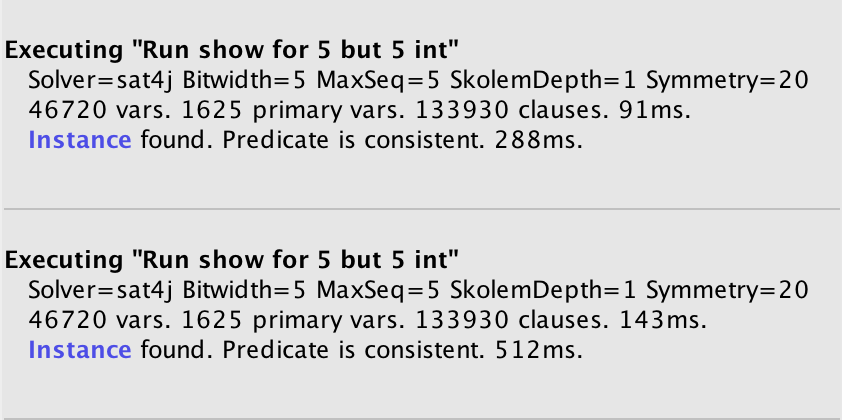
\includegraphics[scale=0.8, origin=c]{executionDetails.png}
        \centering
        \caption{Execution Details}
    \label{fig:execDetail}
\end{figure}

\begin{figure}[H]
        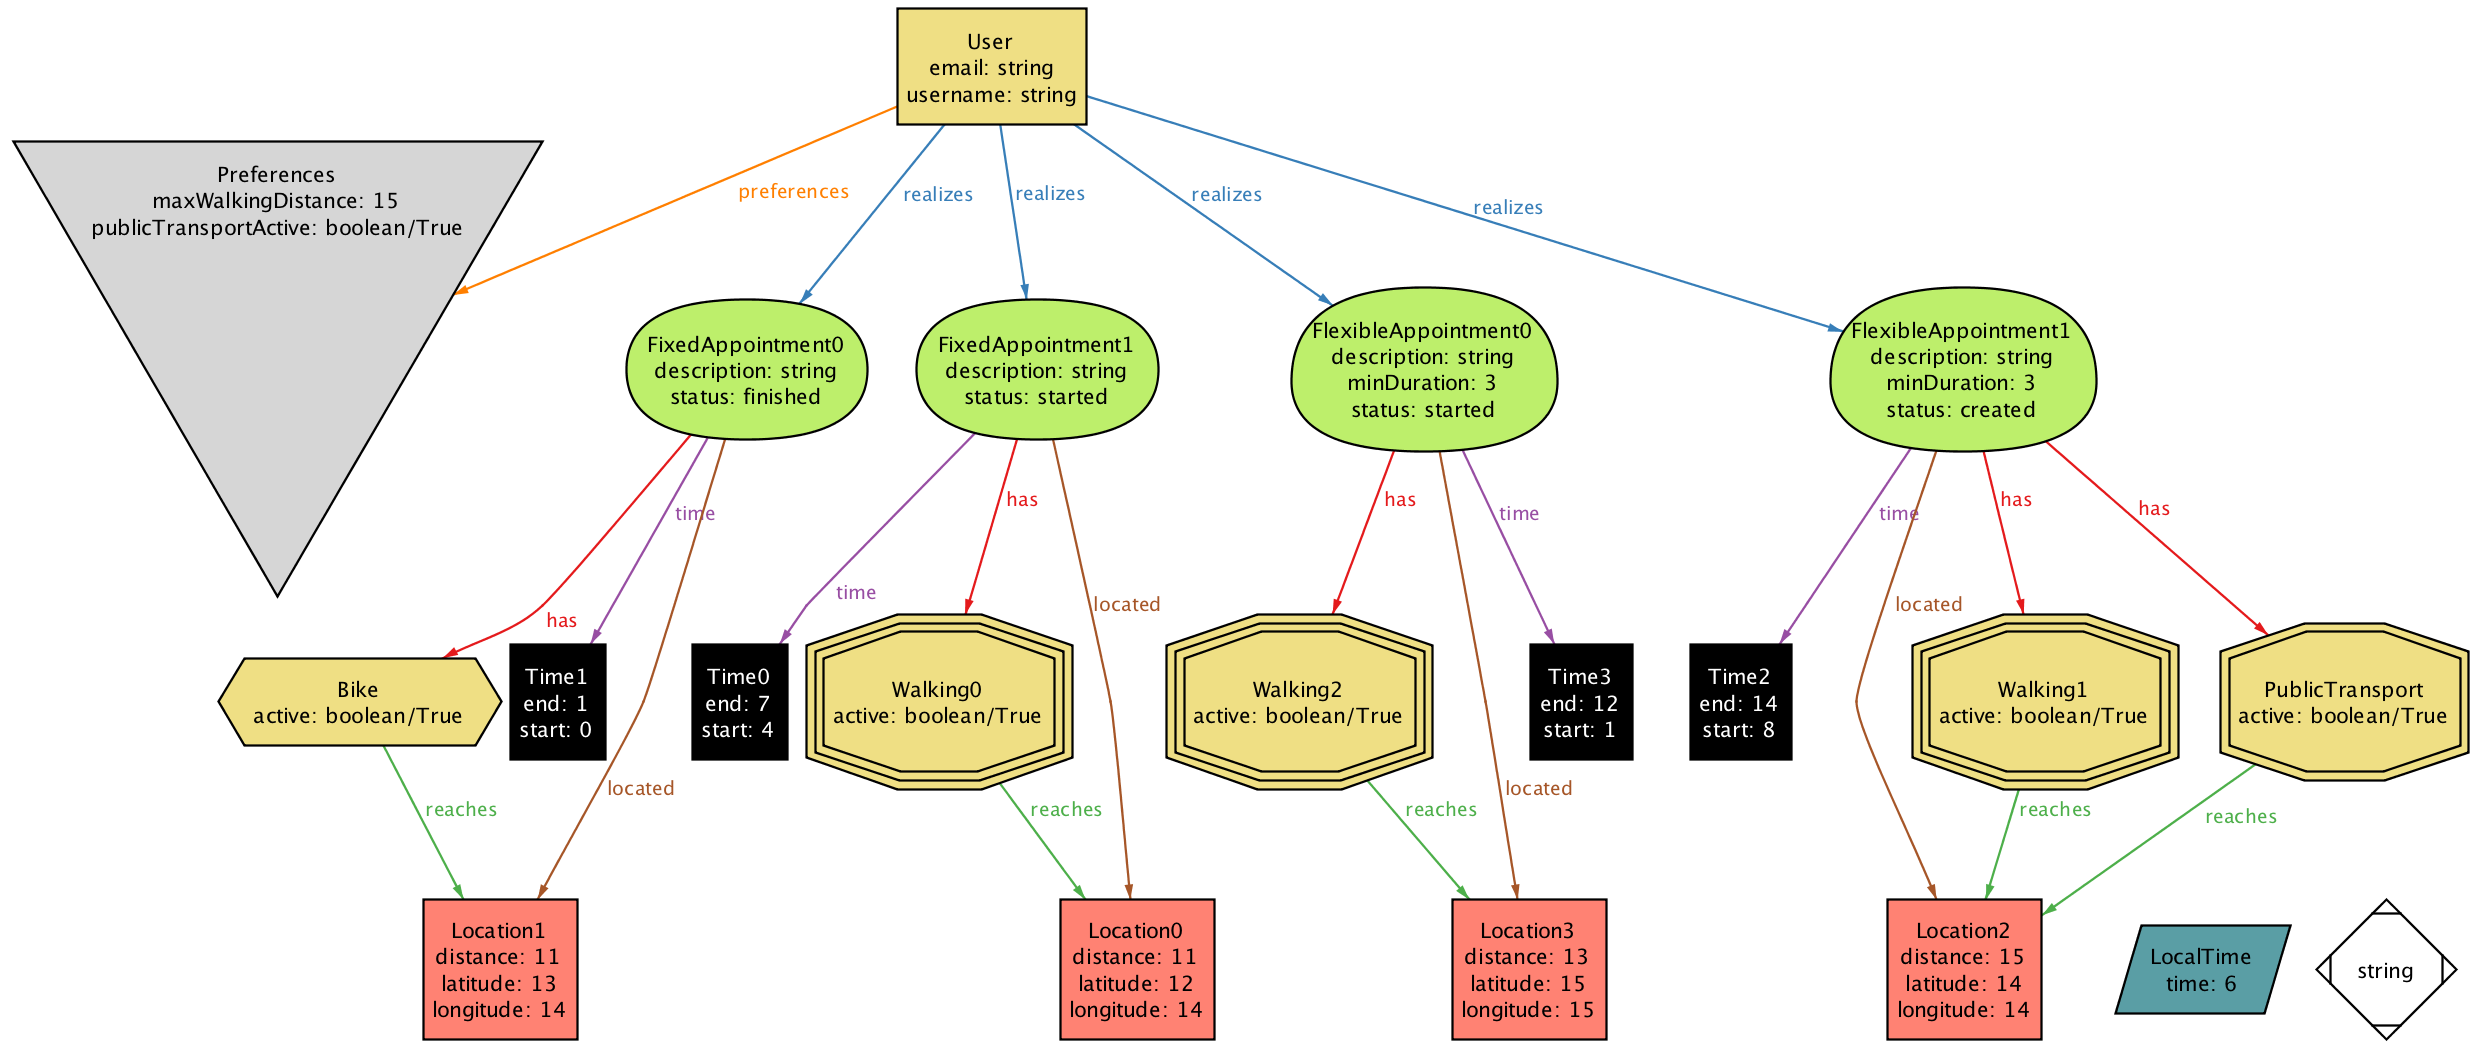
\includegraphics[scale=0.41, angle=-90, origin=c]{generatedWorld1.png}
        \centering
        \caption{Generated World 1}
    \label{fig:execDetail}
\end{figure}

\begin{figure}[H]
        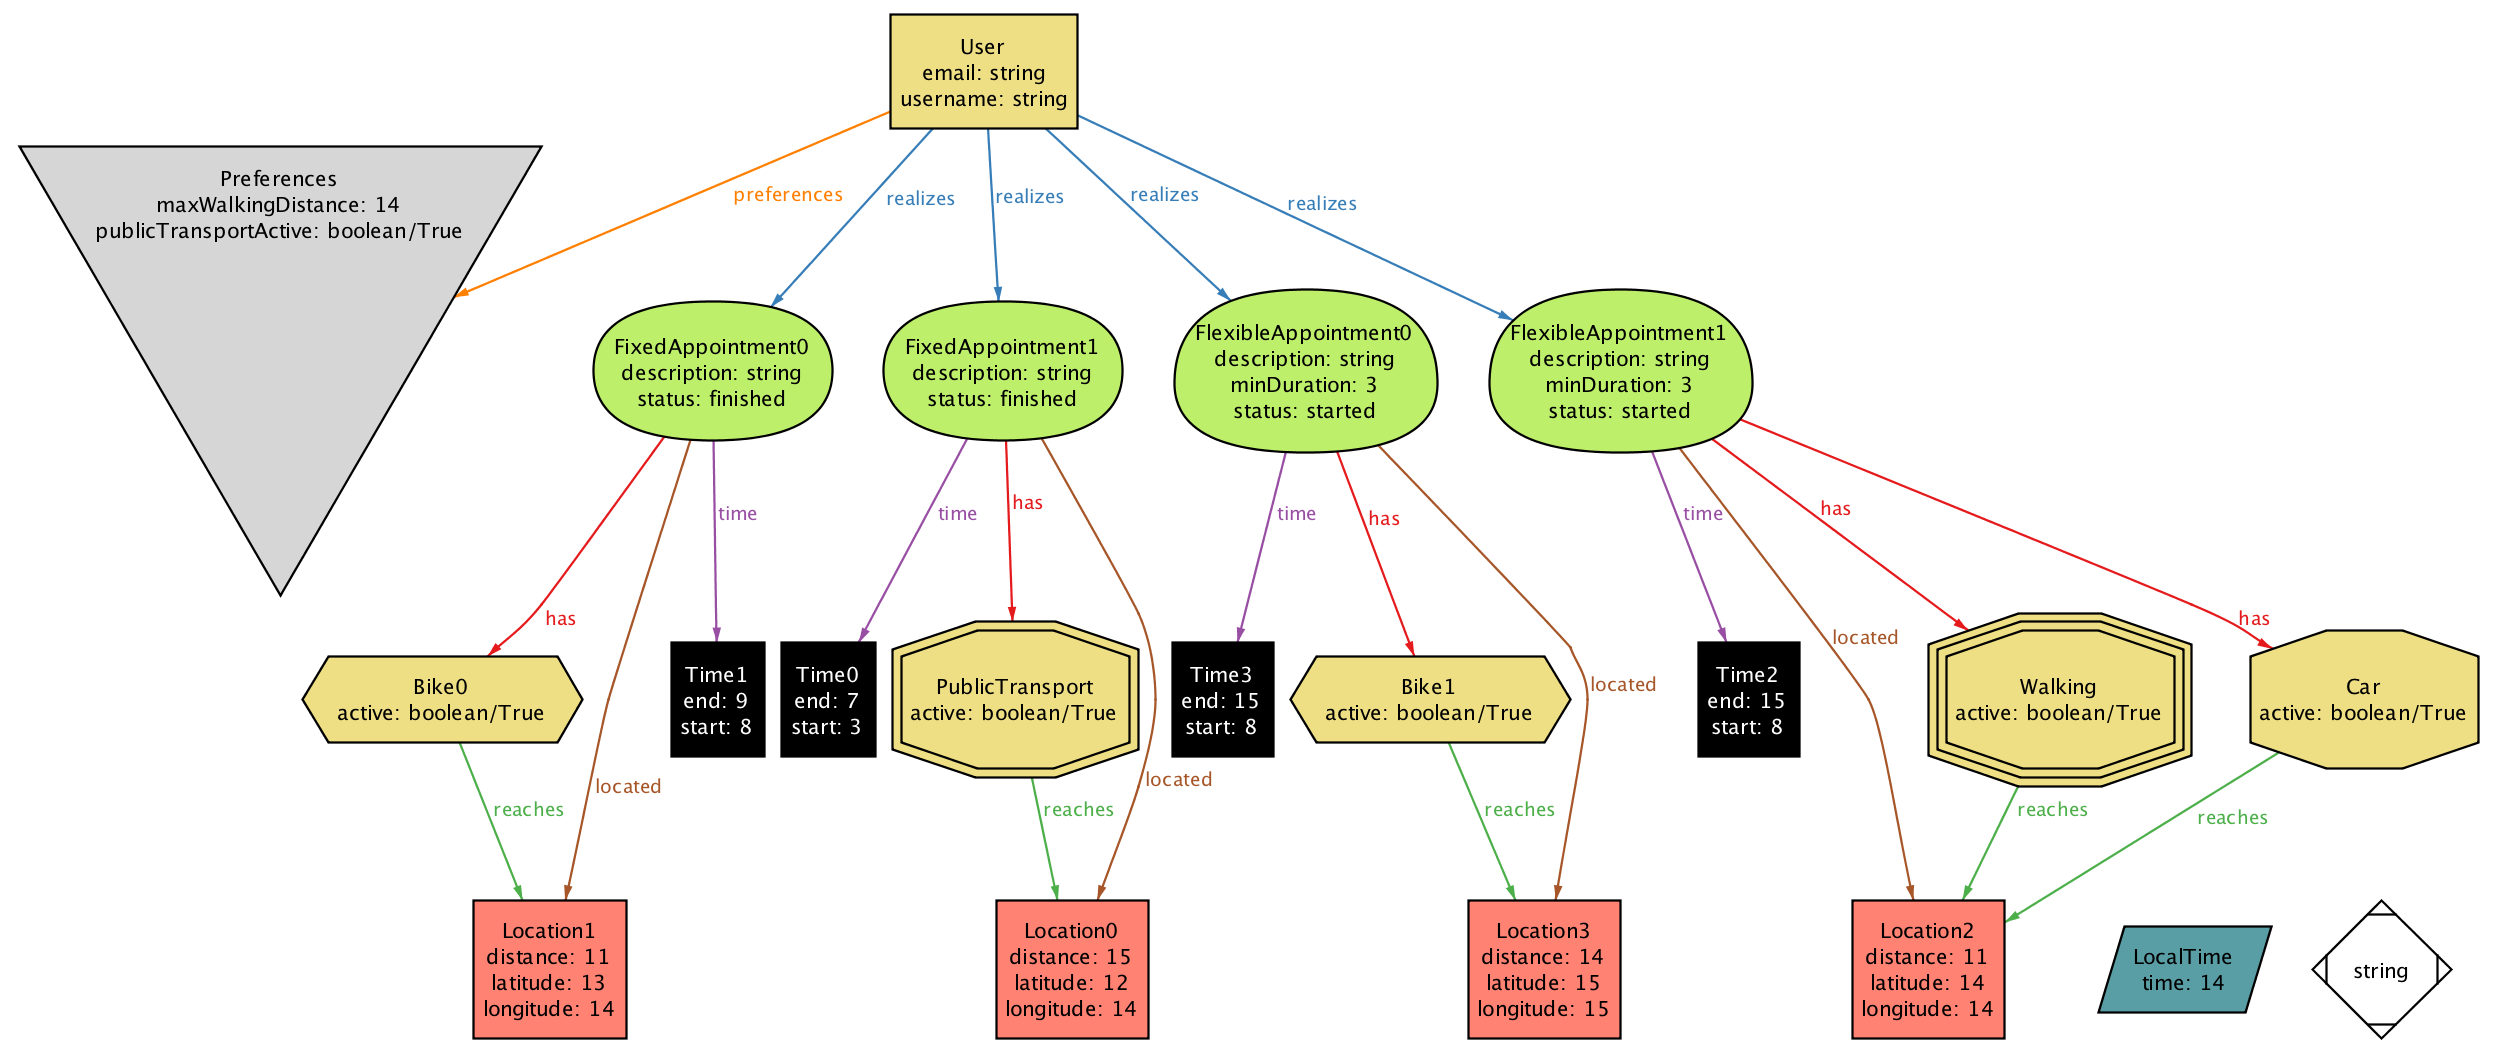
\includegraphics[scale=0.42, angle=-90, origin=c]{generatedWorld2.png}
        \centering
        \caption{Generated World 2}
    \label{fig:execDetail}
\end{figure}

\section{Effort Spent}
\subsection{Francisco Cristóvão}

\begin{center}
\begin{tabular}{ |p{0.25\textwidth}|p{0.4\textwidth}|p{0.25\textwidth}| } 
 \hline
 \textbf{DATE} & \textbf{TASK} & \textbf{HOURS} \\ 
  \hline
 03/10/2017 & Requirements Analysis & 1 \\ 
  \hline
 08/10/2017 & Domain Model and Class Diagram & 1,5 \\ 
  \hline
  09/10/2017 & Purpose and Document Structure & 1 \\ 
  \hline
  11/10/2017 & Scope and Purpose & 1 \\ 
  \hline
  12/10/2017 & User, Software and Hardware Interfaces, Product Functions and User Characteristics & 4,5 \\ 
  \hline
  13/10/2017 & Software System Attributes & 3 \\ 
  \hline
  16/10/2017 & Goals and Requirements, Use case Description & 2 \\ 
  \hline
  17/10/2017 & Use Case Description and User Interface & 4 \\ 
  \hline
  18/10/2017 & Goals, Requirements and Domain Assumptions & 2 \\ 
  \hline
  19/10/2017 & Use Case Description, Performance Constraints & 2 \\ 
  \hline
  20/10/2017 & Goals and requirements, UseCases, UML Diagrams & 3 \\ 
  \hline
  21/10/2017 & BPMN Diagrams, Goals and Requirements, User Interface & 2 \\ 
  \hline
  24/10/2017 & Alloy & 2 \\ 
  \hline
  25/10/2017 & Alloy & 3 \\ 
  \hline
  26/10/2017 & Alloy and General Document Aspects & 3 \\ 
  \hline
  27/10/2017 & Alloy & 6 \\ 
  \hline
  28/10/2017 & Alloy and Final details & 4 \\ 
  \hline
  20/12/2017 & Overall Improvements: creation of version 1.1 & 1,5 \\ 
  \hline
  \textbf{TOTAL} & \multicolumn{2}{c|}{46,5} \\ 
  \hline
\end{tabular}
\end{center}

\subsection{Samsom Tsegay Beyene}

\begin{center}
\begin{tabular}{ |p{0.25\textwidth}|p{0.4\textwidth}|p{0.25\textwidth}| } 
 \hline
 \textbf{DATE} & \textbf{TASK} & \textbf{HOURS} \\ 
  \hline
 03/10/2017 & Requirements Analysis & 2 \\ 
 \hline
 05/10/2017 & First Draft of Scope and Purpose & 2 \\
 \hline
 08/10/2017 & Purpose & 2 \\
 \hline
 10/10/2017 & Document Structure & 3 \\
 \hline
 12/10/2017 & Product Perspective and User Characteristics & 3 \\
 \hline
 13/10/2017 & Communication Interface & 1 \\
 \hline
 14/10/2017 & Use Case Diagrams & 3 \\
 \hline
 16/10/2017 & Goals and Requirements, Use case Description & 2 \\
 \hline
 19/10/2017 & BPMN Diagrams & 2 \\
 \hline
 21/10/2017 & Alloy Signatures & 2 \\
 \hline
 27/10/2017 & RASD Final Review & 2 \\
  \hline
  \textbf{TOTAL} & \multicolumn{2}{c|}{24} \\ 
  \hline
\end{tabular}
\end{center}

\section{Used Tools}
\begin{itemize}
    \item ShareLateX
    \item StarUML 2.8.0
    \item Sketch 47.1
    \item Alloy Analyzer 4.2
\end{itemize}

\section{References}

\begin{thebibliography}{9}
\bibitem{belisoft} 
https://belitsoft.com/php-development-services/software-requirements-specification-document-example-international-standard
\bibitem{portability} 
https://en.wikipedia.org/wiki/Portability\_testing
\bibitem{maintainability} 
https://en.wikipedia.org/wiki/Maintainability
\bibitem{reliability} 
https://en.wikipedia.org/wiki/Software\_reliability\_testing
\bibitem{Nilson} 
Nielsen, Jakob, Budiu, Raluca. \textit{Mobile Usability, 1st Edition}
\bibitem{compliance}
http://www.enforcive.com/regulatory-compliance-software
\bibitem{data}
https://data.oecd.org/pop/working-age-population.htm

\end{thebibliography}
\end{document}